\begin{theorem}
	\hypertarget{thrm5.7}{(Инвариантность формы первого дифференциала и неинвариантность формы высших дифференциалов)} Пусть функция $y = y(x)$ дифференцируема в точке $x_{0},$ а функция $z = z(x)$ дифференцируема в точке $y_{0} = y(x_{0}).$
	
	Тогда дифференциал $z,$ рассматриваемый как функция лишь от $y$ в точке $y_{0},$  и дифференциал функции $z= z(y(x)) = f(x)$ в точке $x_{0}$ записываются одинаково. А именно $dz = z'(y_{0}) \ dy$. При этом в первом случае (когда $z=z(y)$) $dy = y-y_{0}$, а во втором $dy$~---~ дифференциал функции $y(x)$ в точке $x_{0}$
\end{theorem}
\begin{proof}
	Для функции $z = z(y)$ по определению дифференциала 
	
	$$dz(y_{0}) = z'(y_{0}) \ dy, \ dy = y-y_{0}$$
	
	Рассмотрим композицию функций $z = z(y(x)) = f(x)$.
	
	$$dz = f'(x_{0}) \ dx = z'(y(x_{0})) \ y'(x_{0}) \ dx = z'(y(x_{0})) \ dy(x_{0})$$
\end{proof}

\begin{note}
	Для второго дифференциала форма записи не инвариантна.
\end{note}
\begin{proof}
	Действительно, пусть функция $z = z(y)$ дважды дифференцируема в точке $y_{0}$
	
	$$d^{2} = z''(y_{0}) \ (dy)^{2}, \ dy = y-y_{0}$$
	
	Если же $z = z(y(x))$
	
	$$d^{2} z = f''(x_{0}) \ (dx)^{2} = \Bigl( z'(y(x)) \cdot y'(x) \Bigr)' \ (dx)^{2}, \Big|_{x = x_{0}}
	$$
	
	$$
	= \Bigl[z''(y(x)) \cdot (y'(x))^{2} + z'(y(x))\cdot y''(x_{0}) \Bigr] \cdot (dx)^{2} = z''(y_{0}) \cdot (y'(x_{0}))^{2} \cdot (dx)^{2} + z'(y(x_{0})) \cdot y''(x_{0}) \cdot (dx)^{2} =$$
	
	$$
	= z''(y_{0}) (dy)^2 + z'(y_{0}) \ d^{2} y(x_{0})
	$$
\end{proof}

\subsection{Формула Лейбница}
Введём некоторые обозначения: 
$$0! :=1$$
$$ n! := 1 \cdot 2 \cdot \ldots \cdot n, \quad n \in \N $$

$ \relax C_{n}^{k}$~---~ биномиальный коэффициент.
$$ \relax C_{n}^{k} := \cfrac{n!}{k!(n-k)!}$$

Соглашение: $u^{(0)}(x) \equiv u(x)$

\begin{theorem} \hypertarget{thrm5.8}{Формула Лейбница}
	Пусть $\exists u^{(n)}(x_{0}) \in \R $ и $\exists v^{(n)}(x_{0}) \in \R$
	
	Тогда $\exists (u\cdot v)^{n} = \sum\limits_{s=0}^{n} \relax C_{n}^{s} u^{(s)}(x_{0}) \cdot v^{(n-s)}(x_{0})$
\end{theorem}
\begin{proof}
	Докажем по индукции.
	
	База индукции: при $n =1 $ верно (\hyperlink{thrm5.3}{обычное правило дифференцирование произведения}).
	
	Пусть доказано при некотором $k \in \N,$ установим при $k + 1$
	
	То есть мы доказали формулу при $k \in \N$:
	$$(u \cdot v)^{(k)} = \sum\limits_{s=0}^{k} \relax C_{k}^{s} u^{(s)}(x_{0}) \cdot v^{(k-s)}(x_{0}) $$
	
	$$
	(u \cdot v)^{(k+1)} = \Bigg(\sum\limits_{s=0}^{k} \relax C_{k}^{s} u^{(s)}(x) \cdot v^{(k-s)}(x) \Bigg)' \Bigg|_{x=x_{0}} = 
	$$
	$$ =\sum\limits_{s=0}^{k} \relax C_{k}^{s} u^{(s+1)}(x_{0}) \cdot v^{(k-s)}(x_{0}) + \sum\limits_{s=0}^{k} \relax C_{k}^{s} u^{(s)}(x_{0}) \cdot v^{(k-s + 1)}(x_{0}) = (*)
	$$
	Произведем замену индексов: $ s + 1 = j, \ s+ j - 1$
	$$
	(*) = \sum\limits_{j=1}^{k+1} \relax C_{k}^{j-1} u^{(j)}(x_{0}) \cdot v^{(k-j + 1)}(x_{0}) + \sum\limits_{j=0}^{k} \relax C_{k}^{j} u^{(j)}(x_{0}) \cdot v^{(k-j + 1)}(x_{0}) =
	$$
	
	$$
	=  \relax C_{k}^{k} u^{(k+1)}(x_{0}) \cdot v(x_{0}) + \relax C_{k}^{0} u(x_{0}) \cdot v^{(k+ 1)}(x_{0}) + \sum\limits_{j=1}^{k} \Bigl(\relax C_{k}^{j-1} + \relax C_{k}^{j} \Bigr) u^{(j)}(x_{0}) \cdot v^{(k+1 -j)}(x_{0}) = 
	$$
	
	Заметим, что
	
	$
	\relax C_{k}^{k} = \relax C_{k+1}^{k+1} = 1,$
	
	$\relax C_{k}^{0} = \relax C_{k + 1}^{0} = 1,
	$
	
	$
	\relax C_{k}^{j-1} +  \relax C_{k}^{j} = \cfrac{k!}{(j-1)!(k-j + 1)!} + \cfrac{k!}{(j)!(k-j)!} =
	$
	$$
	= \cfrac{k!}{(j)!(k-j+1)!} \cdot ( k -j + 1 + j) = \cfrac{(k+1)!}{(j)!(k+1-j)!} = C_{k+1}^{j}
	$$
	
	С учетом этого перепишем выражение $(*)$
	
	$$
	(u \cdot v)^{(k+1)} = (*) = \sum\limits_{j=0}^{k+1} \relax C_{k+1}^{j} u^{(j)}(x_{0}) \cdot v^{(k+1-j)}(x_{0})
	$$
	
	Шаг индукции доказан. Значит, формула верна при всех $n \in \N.$
\end{proof}

\subsection{Вычисление производных функций, заданных неявно}

\begin{definition}
	Будем говорить, что функция $y: X \mapsto \R$ \textit{неявно задана уравнением} $F(x, y) = 0$, если $F(x,y(x)) = 0 \quad \forall x \in X$  
\end{definition}
\begin{example}
	$$x^2 + y^2 = 1$$
	$$F (x, y) = x^2 + y^2 - 1 $$
	
	$y_{1}(x) = \sqrt{1-x^2}$~---~ функция, неявно заданная уравнением $F (x, y) = 0$
	
	$y_{2}(x) = -\sqrt{1-x^2}$~---~ функция, неявно заданная уравнением $F (x, y) = 0  $
	
	Также заметим, что функций, неявно задающихся данным уравнением, бесконечно много.
\end{example}

\begin{note}
	В домашних задачах априори предполагается, что неявно заданные функции существуют и они дифференцируемы. Однако в общем случае это нужно доказывать.
\end{note}

Чтобы найти производную неявно заданной функции, необходимо:
\begin{enumerate}
	\item Продифференцировать обе части уравнения, вместо $y$ подставляя $y(x)$. Так как оно является тождеством при всех значениях $x$,
	\item Выразить производную $y'(x)$.
\end{enumerate}

\subsection{Производные функций, заданных параметрически}
Пусть $\begin{gathered}
	y = y(t), \\
	x = x(t)
\end{gathered}$ определены в некоторой $U_{\delta}(t_{0})$. 

Если для $x$ выполнены условия, требуемые для \hyperlink{thrm4.19}{теоремы об обратной функции}, то $\exists t = t(x),$ определенная в $U_{delta}(x_{0}),\ x_{0} = x(t_{0}).

Пусть также выполнены все условия \hyperlink{5.11}{ теоремы о дифференцировании обратной функции} и \hyperlink{thrm5.10}{теоремы о дифференцировании сложной функции}. Тогда

$$f(x) = y(t(x))$$

$$y'_{x}(x_{0}) = \cfrac{y'_{t}(t_{0})}{x'_{t}(t_{0})}, \textrm{где} \ t_{0} = t(x_{0})$$

\section{Теоремы о среднем}

\begin{definition}
	Пусть $f : X \mapsto \R, X \subset \R$.
	
	Будем говорить, что точка $x_{0}$~---~ \textrm{точка локального максимума (локального минимума) функции $f$,} если 
	$$\exists \delta = \delta (x_{0}) > 0: \begin{gathered}
		f(x) \leq f(x_{0}) \ \forall x \in U_{\delta}(x_{0}) \cap X\\
		\Bigl( f(x) \geq f(x_{0}) \ \forall x \in U_{\delta}(x_{0}) \cap X\Bigr) 
		\end{gathered}$$
\end{definition}

\begin{definition}
	Пусть $f : X \mapsto \R, X \subset \R$.
	
	Будем говорить, что точка $x_{0}$~---~ \textrm{точка строгого локального максимума (строгого локального минимума) функции $f$,} если 
	$$\exists \delta = \delta (x_{0}) > 0: \begin{gathered}
		f(x) < f(x_{0}) \ \forall x \in \mathring{U}_{\delta}(x_{0}) \cap X\\
		\left( f(x) > f(x_{0}) \ \forall x \in \mathring{U}_{\delta}(x_{0}) \cap X\right) 
	\end{gathered}$$
\end{definition}

\begin{lemma}
	Пусть $f: [a, b] \mapsto \R$. Пусть $x_{0}$~---~ точка локального минимума (локального максимума).
	
	Тогда, если $ \begin{gathered}
		\exists f'_{+} (x_{0}),$ то $ f'_{+} (x_{0}) \geq 0 \\
		\exists f'_{-} (x_{0}),$ то $ f'_{-} (x_{0}) \leq 0 \\
		\left(
		\begin{gathered}
			\exists f'_{+} (x_{0}),$ то $ f'_{+} (x_{0}) \leq 0 \\
			\exists f'_{-} (x_{0}),$ то $ f'_{-} (x_{0}) \geq 0			
		\end{gathered}
		\right)
	\end{gathered}$
\end{lemma}
\begin{proof}
	.
	
	\sidefig(10 cm)(7 cm)	
	{\begin{flushleft}
		
		Докажем для случая, когда $x_{0}$~---~ точка локального минимума, так как для локального максимума доказательство аналогично.	
			
	\end{flushleft}
	}
	{
	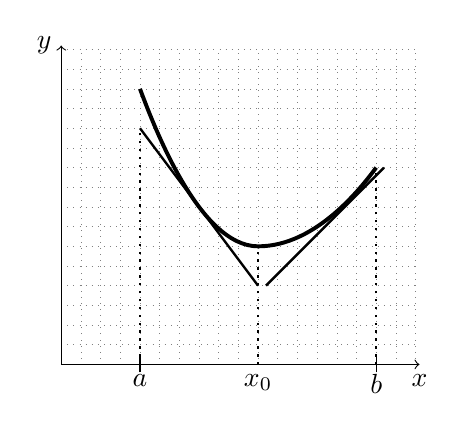
\begin{tikzpicture}
		% Рисуем сетку
		\draw[help lines, step=0.25, dotted]
		(0,0) grid (4.5,4);
		% Начало координат
		\draw[->, thin] (0,0) -- (4.55,0)
		node[below] {$x$}; % Ox
		\draw[->, thin] (0,0) -- (0, 4.05)
		node[left] {$y$}; % Oy
		
		\draw[line width =.05cm](1, 3.5) parabola bend (2.5, 1.5)(4, 2.5);
		
		\draw[line width =.03cm] (1, 3) -- (2.5, 1);
		\draw[line width =.03cm] (2.6, 1) -- (4.1, 2.5);
				
		\draw[dotted, line width =.03cm] (2.5, 0) -- (2.5, 1.5);
		\draw[dotted, line width =.03cm] (1, 0) -- (1, 3);
		\draw[dotted, line width =.03cm] (4, 0) -- (4, 2.5);
		
		\node[below] at (1, 0) {$a$};
		\node[below] at (2.5, 0) {$x_{0}$};
		\node[below] at (4, 0) {$b$};
		
		\draw[thin] (1, -0.1) -- (1, 0.1);
		\draw[thin] (4, -0.1) -- (4, 0.1);
	\end{tikzpicture}
	}
\end{proof}














